%%%%%%%%%%%%%%%%%%%%%%%%%%%%%%%%%%%%%%%%%%%%%%%%%%%%%%%%%%%%%%%%%%%%%%%%%%%%%%%%%%%%%%%%%%%%%%%%%%%
%%%%%%%%%%%%%%%%%%%%%%%%%%%%%%%%%%%%%%%%%%%%%%%%%%%%%%%%%%%%%%%%%%%%%%%%%%%%%%%%%%%%%%%%%%%%%%%%%%%
%%%%%%%%%%%%%%%%%%%%%%%%%%%%%%%%%%%%%%%%%%%%%%%%%%%%%%%%%%%%%%%%%%%%%%%%%%%%%%%%%%%%%%%%%%%%%%%%%%%
%%%%%%%%%%%%%%%%%%%%%%%%%%%%%%%%%%%%%%%%%%%%%%%%%%%%%%%%%%%%%%%%%%%%%%%%%%%%%%%%%%%%%%%%%%%%%%%%%%%

\section{Matemáticas}

%
%El cuerpo central de este trabajo es averiguar sin este modelo de tipo estocástico para los datos
%permite la hipótesis de que los procesos estocásticos involucrados son estacionarios, cuando menos en
%un sentido débil.

Existe una larga tradición en las ciencias biomédicas para entender (y modelar) las señales
electrofisiológicas en términos de ondas y frecuencias, en parte debido a que fundamentalmente son
fenómenos eléctricos \cite{Kaiser00}.
El enfoque que se aborda, a \textit{grosso modo}, es asociar la \textit{energía} de una señal con 
la norma inducida por un producto interno, luego usar una base de un espacio (\textit{componentes 
de frecuencia}) para estudiar cómo se reparte esta energía entre tales elementos;
en concreto,
esto se logrará usando una generalización de la base Fourier para la familia de 
procesos estocásticos \textit{semi-estacionarios}.

Cabe mencionar que se propone como hipótesis que las señales constituyen un fenómeno 
predominantemente estocástico; esto no significa que las señales sean completamente aleatorias, sino 
que el posible no-determinismo está considerado en el modelo.
Por otro lado, aunque las señales sólo son registrables en un conjunto finito de puntos en el 
tiempo, se supone que el fenómeno ocurre efectivamente \textit{a tiempo continuo}, lo cual 
permitirá asumir algunas propiedades para el modelo.

Una vez formulado el modelo descrito, el objetivo principal es estudiar si éste es adecuado (en un 
sentido estadístico) para las señales que conforman el polisomnograma, o si pueden se explicadas
mejor como procesos estocásticos débilmente estacionarios (un modelo más particular). Dado el 
enfoque descrito, la comparación entre modelos se hará \textit{en términos ondas y frecuencias}.

%%%%%%%%%%%%%%%%%%%%%%%%%%%%%%%%%%%%%%%%%%%%%%%%%%%%%%%%%%%%%%%%%%%%%%%%%%%%%%%%%%%%%%%%%%%%%%%%%%%

\subsection{Transformada de Fourier}

La exposición inicia con los espacios de las \textbf{series $\boldsymbol{p}$-sumables}
($\lp$), y las  \textbf{funciones $\boldsymbol{p}$-integrables} sobre un intervalo 
$I \subseteq \R$ ($\llp$).
%; en el presente trabajo sólo se usarán los casos $p=1,2$.
%
%\begin{align}
%\ell^{p} &:= \left\{ s: \Z\rightarrow\C \talque \sum_{n=-\infty}^{\infty} \abso{s(n)}^{p} < \infty \right\}
%\label{lpdef} \\
%L^{p}[I] &:= \left\{ S: I\rightarrow\C \talque \int_I \abso{S(t)}^{p} dt < \infty \right\}
%\label{llpdef}
%\end{align}
\begin{align*}
\ell^{p} &:= \left\{ s: \Z\rightarrow\C \talque \sum_{n=-\infty}^{\infty} \abso{s(n)}^{p} < \infty \right\}
\\
L^{p}[I] &:= \left\{ S: I\rightarrow\C \talque \int_I \abso{S(t)}^{p} dt < \infty \right\}
\end{align*}

Estos espacios admiten las operaciones $+$, $\cdot$ y multiplicación por escalares complejos de la 
manera usual.%, es decir

%\begin{align*}
%s, z \in \lp, c \in \C \Rightarrow 
%[s+z](n) &= s(n) + z(n) \\
%[s\cdot z](n) &= s(n) z(n) \\
%[c \cdot s](n) &= s(n)c \\
%S, Z \in \llp, c \in \C \Rightarrow 
%[S+Z](t) &= S(t) + Z(t) \\
%[S\cdot Z](t) &= S(t)  Z(t) \\
%[c \cdot S](t) &= S(t)c
%\end{align*}
%
%En las próximas líneas se seguirán usando $s, z, S, Z, c$.

Para el caso particular $p=2$, los conjuntos $\ldos$ y $\lldos$ admiten los siguientes productos 
internos:
%
\begin{align*}
\left\langle s,z \right\rangle &= \sum_{n=-\infty}^{\infty} s(n) \overline{z(n)}\\
\left\langle S,Z \right\rangle &= \int_I S(t) \overline{Z(t)} dt
\end{align*}

Usando dichos productos internos, junto con las normas y métricas que inducen, los conjuntos 
$\ldos$ y $\lldos$ tienen estructura de \textbf{espacio de Hilbert}.

Con las definiciones anteriores, que muestran que $\ldos$ y $\lldos$ son \textit{muy}
parecidos, se puede formular unas definición para la transformada de Fourier como una equivalencia
entre estos espacios.

%{De manera pragm\'atica, en el presente trabajo la 
%palabra  'frecuencia' se usar\'a para referirse a la cantidad $q$ en expresiones del tipo 
%$e^{i q t}$}

\begin{definicion}[Serie de Fourier]
Sea $S: \R \rightarrow \C$ una función periódica con periodo $2T$ y tal que 
$S \in L^{2}\left[[-T,T]\right]$. Se dice que $A$ es la serie de Fourier para $S$ si cumple que
\begin{equation*}
A(n) = \frac{1}{2 T} \simint{T} S(t) e^{-\nicefrac{ i \abso{n} t}{2T}} dt
\end{equation*}
%Adicionalmente, la función $\mathcal{F} : \lldos \rightarrow \ldos : S \mapsto A$  recibe el nombre
%de \textbf{Transformada de Fourier}
\label{FourierClasico}
\end{definicion}

\begin{definicion}[Transformada de Fourier]
Sean $S$ y $A$ como en la definición \ref{FourierClasico}. Se le llama transformada de Fourier a la
función $\mathcal{F}_T : L^{2}\left[[-T,T]\right] \rightarrow \ldos : S \mapsto A$
\end{definicion}

Puede interpretarse a $A$ como las \textit{coordenadas} de $S$ en $L^{2}\left[[-T,T]\right]$, 
usando una base de funciones $\left\{ e^{\nicefrac{i \abso{n} t}{2 T}} \right\}_{n\in \Z}$, las
cuales resultan ser ortonormales; esta base en particular es conocida como la \textbf{base de 
Fourier}.
Se demuestra en el anexo A que $\mathcal{F_T}$ está bien definida en el sentido de 
tener efectivamente el dominio y codominio indicados. Así mismo, cabe mencionar las siguientes 
propiedades de $\mathcal{F}_T$
\begin{itemize}
\item Es lineal, es decir, $\mathcal{F}_T[cS + Z] = c\mathcal{F}_T[S] + \mathcal{F}_T[Z]$

\item \textbf{No} es invertible, aunque se le suele definir una
pseudoinversa\footnote{$\mathcal{F}_T^{\text{inv}}$ es \textit{exacta} salvo por la suma
de alguna función $S_0$ tal que $\int_{-T}^{T}\abso{S_0(t)}dt = 0$} como
\begin{equation*}
\mathcal{F}_{T}^{\text{inv}} : \ldos \rightarrow L^{2}\left[[-T,T]\right] :
A \mapsto \sum_{n -\infty}^{\infty} A(n) e^{\nicefrac{i \abso{n} t}{2 T}}
\end{equation*}
\end{itemize}

Con esta terminología se define, de manera pragmática, la \textbf{energía disipada} y la 
\textbf{potencia} de una función $S$ en un intervalo $[a,b]$ como 
\begin{align*}
\text{energía}[S]_{[a,b]} &= \int_a^{b} \abso{S(t)}^{2} dt \\
\text{potencia}[S]_{[a,b]} &= \frac{1}{b-a} \int_a^{b} \abso{S(t)}^{2} dt
\end{align*}
%
%Estas últimas definiciones cobran importancia a la luz del teorema \ref{parseval}: la energía de 
%una función equivale a su norma.

Una consecuencia interesante de este concepto de energía frente al teorema \ref{parseval} es que la 
energía disipada por una función equivale a la suma de la energía disipada por sus 
\textit{componentes} en la base de Fourier.
Conviene, entonces, definir una función que \textit{desglose} estos \textit{aportes}.

\begin{teorema}[Parseval]
Sea $S \in L^{2}\left[[-T,T]\right]$, y sea $A = \mathcal{F}[S]$. Se cumple que
\begin{equation*}
\int_{-T}^{T} \abso{S(t)}^{2} dt = \sum_{n=-\infty}^{\infty} \abso{A(n)}^{2}
\end{equation*}
\label{parseval}
\end{teorema}

\begin{definicion}[Espectro de potencias]
Sea $S \in L^{2}\left[[-T,T]\right]$, y sea $A = \mathcal{F}[S]$. Se llama espectro de potencias 
para $S$ a la función $h_S : \R \rightarrow \R $, definida como
\begin{equation*}
h_S(\omega) = 
\begin{cases}
\abso{A(n)}^{2} & \text{ , si } \omega = \nicefrac{n}{2T}, \text{   con } n\in \mathbb{Z} \\
0 & \text{ ,  otro caso}
\end{cases}
\end{equation*}
\label{espec}
\end{definicion}

Un elemento que será de crucial importancia en el desarrollo posterior es la \textbf{convolución}, 
$\ast$, una tercera operación binaria definida en estos espacios como
%
\begin{align*}
[s \ast z] (\tau) &= \sum_{n=-\infty}^{\infty} s(n) \overline{z(\tau-n)} \\
[S \ast Z] (\tau) &= \int_I S(t) \overline{Z(\tau-t)}
\end{align*}
%
donde $\overline{c}$ es el conjugado complejo de $c$. 
%La convolución es conmutativa y asociativa con la suma. 
Esta operación cobra importancia por la forma en que se relaciona con $\mathcal{F}_T$
%
\begin{teorema}%[de la convolución]
Sean $S,Z \in L^{2}\left[[-T,T]\right]$, entonces se satisface que
\begin{align*}
\mathcal{F}_T[S\ast Z]  &= \mathcal{F}_T[S] \cdot \mathcal{F}_T[Z] \\
\mathcal{F}_T[S\cdot Z] &= \mathcal{F}_T[S] \ast  \mathcal{F}_T[Z] \\
\end{align*}
\label{t_convolucion}
\end{teorema}

\subsubsection{Generalizaciones}

La primera gran generalización sobre la transformada de Fourier es para el conjunto de funciones 
$L^{1}\left[ \R \right]$, definido como en la sección anterior; éste también es un espacio de 
Hilbert usando el producto interno descrito.
La generalización propuesta, teorema \ref{intFourier}, sólo se diferencia en que no se exige que 
la función sea periódica y en el espacio que actúa; 
es quizá más llamativo el que el codominio de $\mathcal{F}_\infty$ no sea $\ldos$ sino $\lldos$,
%es decir que su codominio no son series sino funciones integrables
lo cual afecta cómo deben interpretarse los \textit{componentes de frecuencia generalizados}. La 
discusión pertinente se efectúa en el anexo B.

\begin{definicion}[Integral de Fourier]
Sea $S \in L^{1}\left[\R\right]$. Se dice que $A$ es la integral de Fourier para $S$ si cumple que
\begin{equation*}
A(\omega) = \intR S(t) e^{- i \omega t} dt
\end{equation*}
%Adicionalmente, la función $\mathcal{F} : \lldos \rightarrow \ldos : S \mapsto A$  recibe el nombre
%de \textbf{Transformada de Fourier}
\label{intFourier}
\end{definicion}

\begin{definicion}[Transformada de Fourier]
Sean $S$ y $A$ como en la definición \ref{intFourier}. Se le llama transformada de Fourier a la
función $\mathcal{F}_\infty : L^{1}\left[\R\right] \rightarrow \ldos : S \mapsto A$
\end{definicion}

Una forma de \textit{relacionar} a los $\mathcal{F}_T$ con $\mathcal{F}_\infty$ es tomar una
función $S \in L^{1}\left[\R\right]$ y para cada $T$ definir una continuación periódica de $S$
%, $S_T$
%\begin{equation*}
\begin{center}
$\displaystyle S_T(t) = S(t_0) $, 
%\end{equation*}
con $\displaystyle -T\leq t_0 \leq T$ y $\displaystyle \frac{t-t_0}{2T} \in \Z$
\end{center} 
%
Posteriormente puede hacerse que
%\begin{equation*}
$\lim_{T\rightarrow \infty} \mathcal{F}_T[S_T] = \mathcal{F}_{\infty}$.
%\end{equation*}
%Este proceso suele interpretarse como que $\mathcal{F}_\infty$ es una versión de la transformada
%de Fourier donde se permite que la función sea periódica con periodo infinito,
%%el periodo de la función ($\nicefrac{1}{\text{frecuencia}}$) sea
%%infinitamente grande, 
%o que la distancia entre frecuancias sea infinitamente pequeño.
%
Dado que las funciones definidas en \ref{FourierClasico} y en \ref{intFourier} serán importantes 
en lo que prosigue, conviene introducir una segunda generalización que abarque a ambas, para lo que
se acude al concepto de integrales en el sentido de Lebesgue-Stieltjes (en un anexo)

\begin{definicion}[Integral de Fourier-Stieltjes]
Sea $S: \R\rightarrow \C$. Se dice que $F$ es la integral de Fourier-Stieltjes para $S$ si ésta 
puede escribirse como
\begin{equation*}
S(x) = \intR e^{- i \omega t} dF(\omega)
\end{equation*}
donde la integral está definida en el sentido de Lebesgue-Stieltjes, y la igualdad se cumple
casi en todas partes
%Adicionalmente, la función $\mathcal{F} : \lldos \rightarrow \ldos : S \mapsto A$  recibe el nombre
%de \textbf{Transformada de Fourier}
\label{intFourierStieltjes}
\end{definicion}

%%%%%%%%%%%%%%%%%%%%%%%%%%%%%%%%%%%%%%%%%%%%%%%%%%%%%%%%%%%%%%%%%%%%%%%%%%%%%%%%%%%%%%%%%%%%%%%%%%%

\subsection{Estacionariedad débil}

\begin{definicion}[Proceso estoc\'astico]
Un proceso estocástico \xt es una familia de variables aleatorias reales, 
indexadas por $t \in T$.
\label{proc_estocastico}
\end{definicion}

Respecto al conjunto $T$ que indexa a un proceso estocástico, y que será referido como 
\textit{tiempo}, conviene introducir dos grandes grupos para los mismos
\begin{itemize}
\item \textit{Continuo} si $T$ es un intervalo cerrado
\item \textit{Discreto} si $T$ es de la forma 
$\{ t_0 + n \delta \lvert n \in U \subseteq \mathbb{Z} \}$
\end{itemize}

Los procesos a tiempo discreto contemplan conjuntos finitos e infinitos de puntos en el tiempo.
No se manejan discutirá sobre otros tipos de tiempo en este trabajo.

Como notación, se usará \xt  para el proceso estocástico y $X(t)$ para una de las variables
aleatorias que lo componen; de la misma manera $x(t)$ es una realización de $X(t)$ y $F_{X(t)}$ 
es la función de probabilidad acumulada para $X(t)$.

\begin{definicion}[Estacionariedad débil]
Un proceso estocástico \xt es débilmente estacionario si y sólo si para cualesquiera tiempos 
admisibles\footnote{El término \textit{tiempos admisibles} significa que la definición es la misma
para diferentes tipos de tiempo, bajo las restricciones pertinente} $t$, $s$ se tiene que
\begin{itemize}
\item $\E{X(t)} = \mu_X$
\item $\Var{X(t)} = \sigma^{2}_X$
\item $\Cov{X(t),X(s)} = \rho_X (s-t)$
\end{itemize}
Donde $\mu_X$, $\sigma^{2}_X$ son constantes, $\rho_X(\tau)$ es una función que únicamente 
depende de $\tau$
\label{est_orden_primera}
\end{definicion}

Adicionalmente se supondrá que las señales en el electroencefalograma (EEG) son continuas, cuando menos
el sentido de media cuadrática

\begin{definicion}[Continuidad estocástica en media cuadrática]
Un proceso estocástico a tiempo continuo $\{ X(t) \}$ es estocásticamente continuo, en el 
sentido de media cuadrática, en un tiempo admisible $t_0$ si y sólo si
\begin{equation*}
\lim_{t \rightarrow t_0} \E{\left( X(t) - X(t_0) \right)^{2}} = 0
\end{equation*}
\label{cont_est}
\end{definicion}

\subsubsection{Función de densidad espectral}

\begin{definicion}[Función de densidad espectral (FDE)]
Sea $\{X(t)\}$ un proceso estocástico en tiempo continuo, débilmente estacionario. Se define la 
función de densidad espectral (FDE) para $\{X(t)\}$ como
%\begin{equation*}
%h(\omega) = \lim_{T\rightarrow \infty} \E{ \frac{ \left| G_T(\omega) \right|^{2}}{2 T} }
%\end{equation*}
\begin{equation*}
h(\omega) = \lim_{T\rightarrow \infty} \E{ \frac{1}{2T} \frac{1}{2 \pi}
\abso{ \int_{-T}^{T} X(t) e^{-i \omega t} dt}^{2} }
\end{equation*}
%Donde $G_T (\omega) = \frac{1}{\sqrt{2 \pi}} \int_{-T}^{T} X(t) e^{-i \omega t} dt$
\label{FDE}
\end{definicion}

\begin{definicion}[Función de espectro integrado]
Sea $\{X(t)\}$ un proceso estoc\'astico a tiempo continuo, débilmente estacionario. Se define la 
función de espectro integrado para $\{X(t)\}$ como
\begin{equation*}
H(\omega) = \int_{-\infty}^{\omega} h(\lambda) d\lambda
\end{equation*}
Donde $h$ es la función de densidad espectral para $\{X(t)\}$
\label{FDE_integrado}
\end{definicion}

Si la FDE, $h$, est\'a bien definida en todos sus puntos, entonces la función de espectro 
integrado ($H$) satisface que $H\prima= h$ y se dirá que el proceso tiene un \textbf{espectro 
puramente continuo}; si $H$ tiene una forma escalonada, con escalones rectos, se dirá que es un 
\textbf{espectro puramente discreto}.
Como es de esperarse, cada tipo de proceso tiene característica diferentes y se puede estudiar 
mejor con herramientas diferentes; para el caso de procesos con un espectro mixto (ninguno de los 
anteriores), se exhiben herramientas que los reducen a estos casos 'puros'.

Cabe destacar que, por como se definió la FDE integrada, ésta es una función positiva, 
no-decreciente, y que en $-\infty$ vale 0; esta observación será importante.

\begin{teorema}[Wiener-Khinchin]
Una condición suficiente y necesaria para que $\rho$ sea una función de autocorrelación de 
algún proceso estocástico a tiempo continuo $\{X(t)\}$ débilmente estacionario y 
estocásticamente continuo, es que exista una función $F$ que tenga las siguientes propiedades
\begin{itemize}
\item Monótonamente creciente
\item $F(-\infty) = 0$
\item $F(+\infty) = 1$
\end{itemize}
y tal que para todo $\tau \in \R$ se cumple que
\begin{equation*}
\rho(\tau) = \intR e^{i \omega \tau} dF(\omega)
\end{equation*}
\label{t_wienerkhinchin}
\end{teorema}

\begin{teorema}[Wold]
Una condición suficiente y necesaria para que $\rho$ sea una función de autocorrelación de 
algún proceso estocástico a tiempo discreto $\{X(t)\}$ débilmente estacionario es que exista 
una función $F$ con las siguientes propiedades
\begin{itemize}
\item Monótonamente creciente
\item $F(-\pi) = 0$
\item $F(+\pi) = 1$
\end{itemize}
y tal que para todo $\tau \in \R$ se cumple que
\begin{equation*}
\rho(\tau) = \intPI e^{i \omega \tau} dF(\omega)
\end{equation*}
\label{t_wold}
\end{teorema}

\subsection{Representación espectral}

\begin{teorema}
Sea $\{X(t)\}$ un proceso estocástico a tiempo continuo débilmente estacionario de media 0 y 
estocásticamente continuo en el sentido de media cuadrática. Entonces, existe un proceso 
ortogonal $\{Z(\omega)\}$ tal que, para todo tiempo $\omega$ admisible, se puede 
escribir\footnote{La integral se encuentra definida en el sentido de media cuadrática.}
\begin{equation*}
X(t) = \intR e^{i t \omega} dZ(\omega)
\end{equation*}
Donde el proceso $\{Z(t)\}$ tiene las siguientes propiedades para todo $\omega$
\begin{itemize}
\item $\E{dZ(\omega)} = 0$
\item $\E{\abso{dZ(\omega)}^{2}} = dH(\omega)$
\item $\Cov{dZ(\omega),dZ(\lambda)} = 0 \Leftrightarrow \omega \neq \lambda$
\end{itemize}
Donde $dH(\omega)$ la FDE integrada de $\{X(t)\}$
\label{rep_espectral}
\end{teorema}

En virtud del teorema de Wold, se puede tener una variante del teorema \ref{rep_espectral}
para procesos a tiempo discreto, razón por la cual  
tal representación es referida como \textbf{representación de Wold-Cramér}.

%%%%%%%%%%%%%%%%%%%%%%%%%%%%%%%%%%%%%%%%%%%%%%%%%%%%%%%%%%%%%%%%%%%%%%%%%%%%%%%%%%%%%%%%%%%%%%%%%%%

\subsection{Estimación}

Conviene introducir estimadores para la función de autocovarianza de un proceso débilmente 
estacionario, $\{ X(t) \}$, a partir de un conjunto de $N$ observaciones equiespaciadas en el 
tiempo con separación $\Delta t$; se denotará a estas observaciones como 
$x_1, x_2 , \dots, x_N$. Como se cumple la siguiente propiedad para la función de autocovarianza, 
$R$, por definición
\begin{equation*}
R(\tau) = \E{X(n\Delta t)X(n\Delta t + \tau)} \text{  ,  } n = 0, 1, 2,  3,\dots, N
\end{equation*}
el estimados estándar para $R$ está dado por la siguiente expresión
\begin{equation*}
\widehat{R}(\tau) = \frac{1}{N-\abso{\tau}} 
\sum_{t = 1}^{N-\abso{\tau}} x_t x_{t+\abso{\tau}}
\label{estimador_R}
\end{equation*}

Se puede demostrar que $\widehat{R}$ es un estimador insesgado\footnote{Un estimador para el 
parámetro $\theta$, $\widehat{\theta}$, se dice \textbf{insesgado} si 
$\E{\widehat{\theta}}=\theta$} y consistente\footnote{Un estimador para el parámetro $\theta$ que 
depende de $N$ observaciones, 
$\widehat{\theta}_N$, se dice \textbf{consistente} si 
$\lim_{N\rightarrow \infty} \Var{\widehat{\theta}_N} = 0$} 
para $R$; sin embargo conviene introducir un estimador diferente para $R$
\begin{equation*}
\aste{R}(\tau) = \frac{1}{N} 
\sum_{t = 1}^{N-\abso{\tau}} x_t x_{t+\abso{\tau}}
\label{estimador_R_ast}
\end{equation*}

\begin{teorema}
Sean $x_1, x_2 , \dots, x_N$ observaciones de un proceso estocástico de media cero y varianza
finita. Se puede calcular el periodograma para estos datos como
\begin{equation*}
I_N(\omega) = 2 \sum_{r = -(N-1)}^{N-1} \aste{R}(r) \COS{r \omega}
\end{equation*}
Donde $\aste{R}$ es el estimador para la función de autocovarianza del proceso, calculado como
$\widehat{R}(\tau) = \frac{1}{N-\abso{\tau}} \sum_{t = 1}^{N-\abso{\tau}} x_t x_{t+\abso{\tau}}$
\label{periodograma_rho}
\end{teorema}

Se puede demostrar que el periodograma es un estimador insesgado de la FDE para los proceso 
considerados; sin embargo, si el proceso tuviera un espectro puramente continuo, ocurre que 
$\lim_{N\rightarrow \infty} \Var{I_N(\omega)} = h^{2}(\omega)$, con $h$ la FDE del proceso: el 
periodograma, en general, no es consistente.
En parte esto ocurre porque el periodograma depende de los estimadores para la función de 
autocovarianza, $\est{R}$, evaluada en todos los puntos posibles: para calcular $\est{R}$ en 
valores muy altos se requieren puntos muy alejados, los cuales son menos abundantes e implican 
una mayor varianza.

Si efectivamente el periodograma aumenta su varianza cuando incluye las 'colas' de la función de 
autocovarianza, entonces una solución es evitarlas, multiplicando por una función de pesos. 
Tales consideraciones dan origen a estimadores de la forma
\begin{equation*}
\est{h}(\omega) = \frac{1}{2\pi} \sum_{s = -(N-1)}^{N-1} 
\lambda(s) \aste{R}(s) e^{i \omega t}
\label{ventaneando}
\end{equation*}
donde la función de pesos, $\lambda$, es referida como \textbf{ventana de retrasos}. Para 
estudiar las propiedades estos estimadores, conviene reescribirlos en función del periodograma

\begin{equation*}
\est{h}(\omega) = \intPI I_N(\theta) W(\omega-\theta) d\theta
\end{equation*}
donde $W$ es la transformada de Fourier finita de $\lambda$
\begin{equation*}
W(\theta) = \frac{1}{2\pi} \sum_{s = -(N-1)}^{N-1} \lambda(s) e^{-is\theta}
\end{equation*}

Cabe destacar la forma que adopta $\est{h}$ como la convolución $I_N \ast W$, que bien puede 
entenderse como que $W$ es una función de pesos en el 'dominio de las frecuencias'; por ello, $W$ 
es referida como \textbf{ventana de retrasos}.
En la tabla \ref{ventanas} hay una lista corta de algunas funciones tipo ventana. Estos estimadores 
son consistentes y sesgados, aunque son asintóticamente insesgados.

%%%%%%%%%%%%%%%%%%%%%%%%%%%%%%%%%%%%%%%%%%%%%%%%%%%%%%%%%%%%%%%%%%%%%%%%%%%%%%%%%%%%%%%%%%%%%%%%%%%

\begin{proposicion}
Sean $u$ y $v$ dos funciones tipo \textit{pseudo $\delta$ de Dirac}, es decir, unimodales con un
máximo  y (...). Si $u$ tiene una concentración muy alta, con relación a $v$, entonces
\begin{equation*}
\intR u(x) v(x+k) dx \approx v(k) \intR u(x) dx
\end{equation*}
\label{pseudo_d}
\end{proposicion}

%%%%%%%%%%%%%%%%%%%%%%%%%%%%%%%%%%%%%%%%%%%%%%%%%%%%%%%%%%%%%%%%%%%%%%%%%%%%%%%%%%%%%%%%%%%%%%%%%%%

\subsection{Estimador de doble ventana}

Respecto a la estimación del espectro local se usa el \textbf{estimador de doble ventana}, 
técnica introducida por Priestley \cite{Priestley69} y que requiere dos funciones, $w_\tau$ y 
$g$, que funcionan como ventana de retrasos y como filtro lineal, respectivamente.
%
En cuando a $g$, se define a $\Gamma(u) = \intR g(u) e^{i u \omega} du$ y se les pide que
\begin{equation*}
2\pi \int_{-\infty}^{\infty} \lvert g(u) \lvert^{2} du 
= 
\int_{-\infty}^{\infty} \lvert \Gamma(\omega) \lvert^{2} d\omega
= 1
\end{equation*}

Cabe mencionar que las ventanas espectrales mostradas en la tabla \ref{ventanas} bien 
pueden cumplir las propiedades requeridas para ser filtros.
Posteriormente se define el estimador $U$ con el objetivo de asignar pesos en el tiempo para estimar
a la FDE
% en el tiempo dado; más aún, $U$ sirve 
%como una aproximación de la representación de Wold-Cramér para 
%el proceso.
\begin{equation*}
U(t,\omega) = \int_{t-T}^{t} g(u) X({t-u}) e^{i \omega (t-u)} du
\end{equation*}

Bajo el entendido que la función $\Gamma$ converge a una función tipo \dirac, puede 
considerarse que 
$\E{\abso{U(t,\omega)}^{2}} \approx f_t(\omega)$; sin embargo, se demuestra en \cite{Priestley66} 
que $\Var{\abso{U(t,\omega)}^{2}} \nrightarrow 0$.
%
Debido a ello se usa una segunda función tipo ventana,
%, para 'suavizar' el estimador y hacerlo consistente (
de forma similar al periodograma.
Se considera la función $W_\tau$, ventana de retrasos, y su respectiva ventana espectral 
$w_\tau$; deben satisfacer las siguientes propiedades:
\begin{itemize}
\item $w_{\tau}(t) \geq 0$ para cualesquiera $t$, $\tau$
\item $w_{\tau}(t) \rightarrow 0$ cuando $\lvert t \lvert \rightarrow \infty$, para todo $\tau$
\item $\displaystyle \int_{-\infty}^{\infty} w_{\tau}(t) dt = 1$ para todo $\tau$
\item $\displaystyle \int_{-\infty}^{\infty} \left( w_{\tau}(t) \right)^{2} dt < \infty$ para todo $\tau$
\item $\exists C$ tal que  
$\displaystyle \lim_{\tau\rightarrow\infty} \tau \int_{-\infty}^{t} \abso{ W_{\tau}(\lambda) }^{2} d\lambda = C$
\end{itemize}

%Por ejemplo, la ventana de Daniell satisface estas propiedades; para ello, conviene calcular que
%$\lim_{\tau\rightarrow\infty} \tau \int_{t-T}^{t} \lvert W_{\tau}(\lambda) \lvert^{2} d\lambda = 2\pi$;
%más aún, 
Cabe mencionar que todas las ventanas mostradas en \ref{ventanas} satisfacen las propiedades 
anteriores.
Finalmente, se define el estimador $\est{f}$ para las FDE normalizada, $f_t$, como
\begin{equation*}
\widehat{f}(t,\omega) = \int_{t-T}^{t} w_{T'}(u) \lvert U(t-u,\omega) \lvert^{2} du
\label{estimador_doble_ventana}
\end{equation*}

Fue demostrado por Priestley \cite{Priestley65} que los estimadores de doble ventana son 
asintóticamente insesgados y consistentes, y propone las siguientes aproximaciones:
%conviene exhibir las siguientes expresiones aproximadas propuestas en aquél trabajo
\begin{itemize}
\item $\displaystyle
\E{\est{f}(t,\omega)} \approx 
\intR \widetilde{f}(t,\omega+\theta) \abso{\Gamma(\theta)}^{2} d\theta$
\item $\displaystyle
\Var{\est{f}(t,\omega)} \approx \frac{C}{\tau} \left( \overline{f}^{2}(\omega) \right)
\intR \abso{\Gamma(\theta)}^{4} d\theta $
\end{itemize}

donde las funciones $\widetilde{f}$ y $\overline{f}$ son versiones 'suavizadas' de la FDE 
normalizada, $f$, y están definidas de la siguiente manera
\begin{equation*}
\widetilde{f}(t,\omega+\theta) = 
\intR W_{\tau}(u) f(t-u,\omega+\theta) du
\end{equation*}
\begin{equation*}
\overline{f}^{2} (t,\omega) =
\frac{\intR f^{2}\left(t-u,W_{\tau}^{2}(u)\right) du}
{\intR \left( W_{\tau}(u) \right)^{2} du}
\end{equation*}

Como $W_{\tau}$ funciona como ventana espectral, converge a una 
función tipo \dirac; luego $\widetilde{f}$ es aproximadamente la convolución 
$\widetilde{f}(t,\omega+\theta) \approx \delta_t \ast f(\bullet,\omega+\theta)$. 
Una aproximación muy similar 
puede hacerse respecto al segundo término, de modo que $\widetilde{f}\approx f$ y 
$\overline{f}^{2}\approx f^{2}$.
Tales aproximaciones serán mejores en tanto las ventanas $w_{\tau}$ y $W_{\tau}$ sean más 
cercanas a funciones tipo \dirac.
%; más aún, una condición adecuada es que estas funciones 
%tengan una forma 'más delgada' que el espacio entre los tiempos y frecuencias donde se estimará 
%$f$.
Dicho esto, se pueden hacer las siguientes aproximaciones, un poco más arriesgadas:
\begin{itemize}
\item $\displaystyle \E{\est{f}(t,\omega)} \approx f(t,\omega)$
\item $\displaystyle \Var{\est{f}(t,\omega)} \approx 
\frac{C}{\tau} f^{2}(t,\omega) \intR \abso{\Gamma (\theta)}^{4} d\theta$
\end{itemize}

\subsection{Prueba de Priestley-Subba Rao}

Una propiedad interesante de poder estimar el espectro evolutivo de un proceso, a partir de una 
realización del mismo, es la capacidad para identificar si éste pudiera reducirse al espectro 
usual, definido para procesos débilmente estacionarios --bastaría con revisar si el espectro 
estimado es constante en el tiempo.
%En otras palabras, el espectro evolutivo puede usarse como herramienta para decidir si un proceso 
%es estacionario.

La prueba de estacionariedad propuesta por Priestley y Subba Rao en 1969 \cite{Priestley69} tiene 
como \textit{ingrediente principal} un estimador muy particular para una cantidad que depende del 
espectro, con propiedades estadísticas adecuadas para detectar la posible estacionariedad.

Sea \xt que se tiene un proceso semi-estacionario y sea \xtd un conjunto de observaciones del 
proceso, espaciadas uniformemente en el tiempo.
Se construye a $\widehat{f}$, el estimador de doble ventana definido como en la sección anterior,
usando las funciones ventana $g_h$ y $w_\tau$, y sus respectivas transformadas de Fourier 
$\Gamma_h$ y $W_\tau$. Como se mencionó previamente, bajo las condiciones descritas se cumple que 
$\widehat{f}$ es un estimador consistente y aproximadamente insesgado para $f$, el espectro
evolutivo de \xt. Ahora bien, considerando las siguientes aproximaciones
%
\begin{itemize}
\item $\E{\widehat{f}(t,\omega)} \approx f(t,\omega)$
\item $\Var{\widehat{f}(t,\omega)} \approx 
\frac{C}{T} f^{2}(t,\omega) \intR \abso{\Gamma^{4}(\theta)} d\theta$
\end{itemize}
%
donde $C = \lim_{T\rightarrow \infty} T \intR \abso{W_T(\lambda)} d\lambda$.
Usando a $\widehat{f}$, se define el estimador $Y$ como el logaritmo de éste, 
$Y(t,\omega) = \log\left(\widehat{f}(t,\omega)\right)$, y que tiene las siguientes propiedades
%
\begin{itemize}
\item $\E{Y(t,\omega)} \approx \log\left(f(t,\omega)\right)$
\item $\Var{Y(t,\omega)} \approx 
\frac{C}{T} \intR \abso{\Gamma_h(\theta)}^{4} d\theta =: \sigma^{2}$
\end{itemize}
%

Cabe destacar que la varianza $Y$ no es formalmente independiente de $f$ sino que es 
\textit{aproximadamente independiente}, es decir, la varianza de $Y$ depende \textit{más} 
del propio estimador que del verdadero valor de $\log\circ f$.
Esto no es tan sorprendente tomando en cuenta el diseño del estimador de doble ventana, que otorga 
mayor importancia a la información local usando repetidamente la proposición \ref{pseudo_d}. Esta 
independencia asintótica sugiere que $Y$ puede verse como
%
%\begin{equation}
$Y(t,\omega) = \log\left(f(t,\omega) \right) + \varepsilon(t,\omega)$,
%\end{equation}
%
con $\E{\varepsilon(t,\omega)} \approx 0$ y $\Var{\varepsilon(t,\omega)} \approx \sigma^{2}$.

Más aún, es demostrado en \cite{Priestley66} que si $\abso{\omega-\omega_0}$ es suficientemente 
grande como para que 
$\intR \abso{\Gamma_h(\theta+\omega)}^{2}\abso{\Gamma_h(\theta+\omega_0)}^{2} d\theta \approx 0$,
entonces 
%
%\begin{itemize}
%\item 
$\Cov{Y(t,\omega),Y(t,\omega_0)} \approx 0$.
%\end{itemize}
%
Similarmente, si $\abso{t-t_0} >> \intR \abso{t} \abso{w_\tau (t)} dt $, entonces
%
%\begin{itemize}
%\item 
$\Cov{Y(t,\omega),Y(t_0,\omega)} \approx 0$.
%\end{itemize}

Bajo estas nuevas condiciones, es posible construir una versión discretizada de $Y$ tal que los 
componentes $\varepsilon$ sean estadísticamente independientes. Para ello se define una malla de 
puntos $(t_i,\omega_j)$, con $i = 1,\dots,I$ y  $j=1,\dots,J$, y posteriormente a la matriz $Y$ 
como $Y_{i,j} = Y(t_i,\omega_j)$, que satisface
%
\begin{itemize}
\item $Y_{i,j} = \log\left(f(t_i,\omega_j)\right) + \varepsilon_{i,j}$
\item $\E{\varepsilon_{i,j}} \approx 0$
\item $\Var{\varepsilon_{i,j}} \approx \sigma^{2} = 
\frac{C}{T} \intR \abso{\Gamma_h(\theta)}^{4} d\theta$
\item $\Cov{\varepsilon_{i,j},\varepsilon_{i_0,j_0}} \approx 0$ siempre que $(i,j)\neq (i_0,j_0)$
\end{itemize}

Ha sido sugerido por Jenkins [??] que si el número de puntos es suficientemente grande, entonces
las componentes de $Y$ siguen distribuciones aproximadamente normales, de modo que
$\varepsilon_{i,j} \sim N(0,\sigma^{2})$.

%\begin{figure}
%\centering
%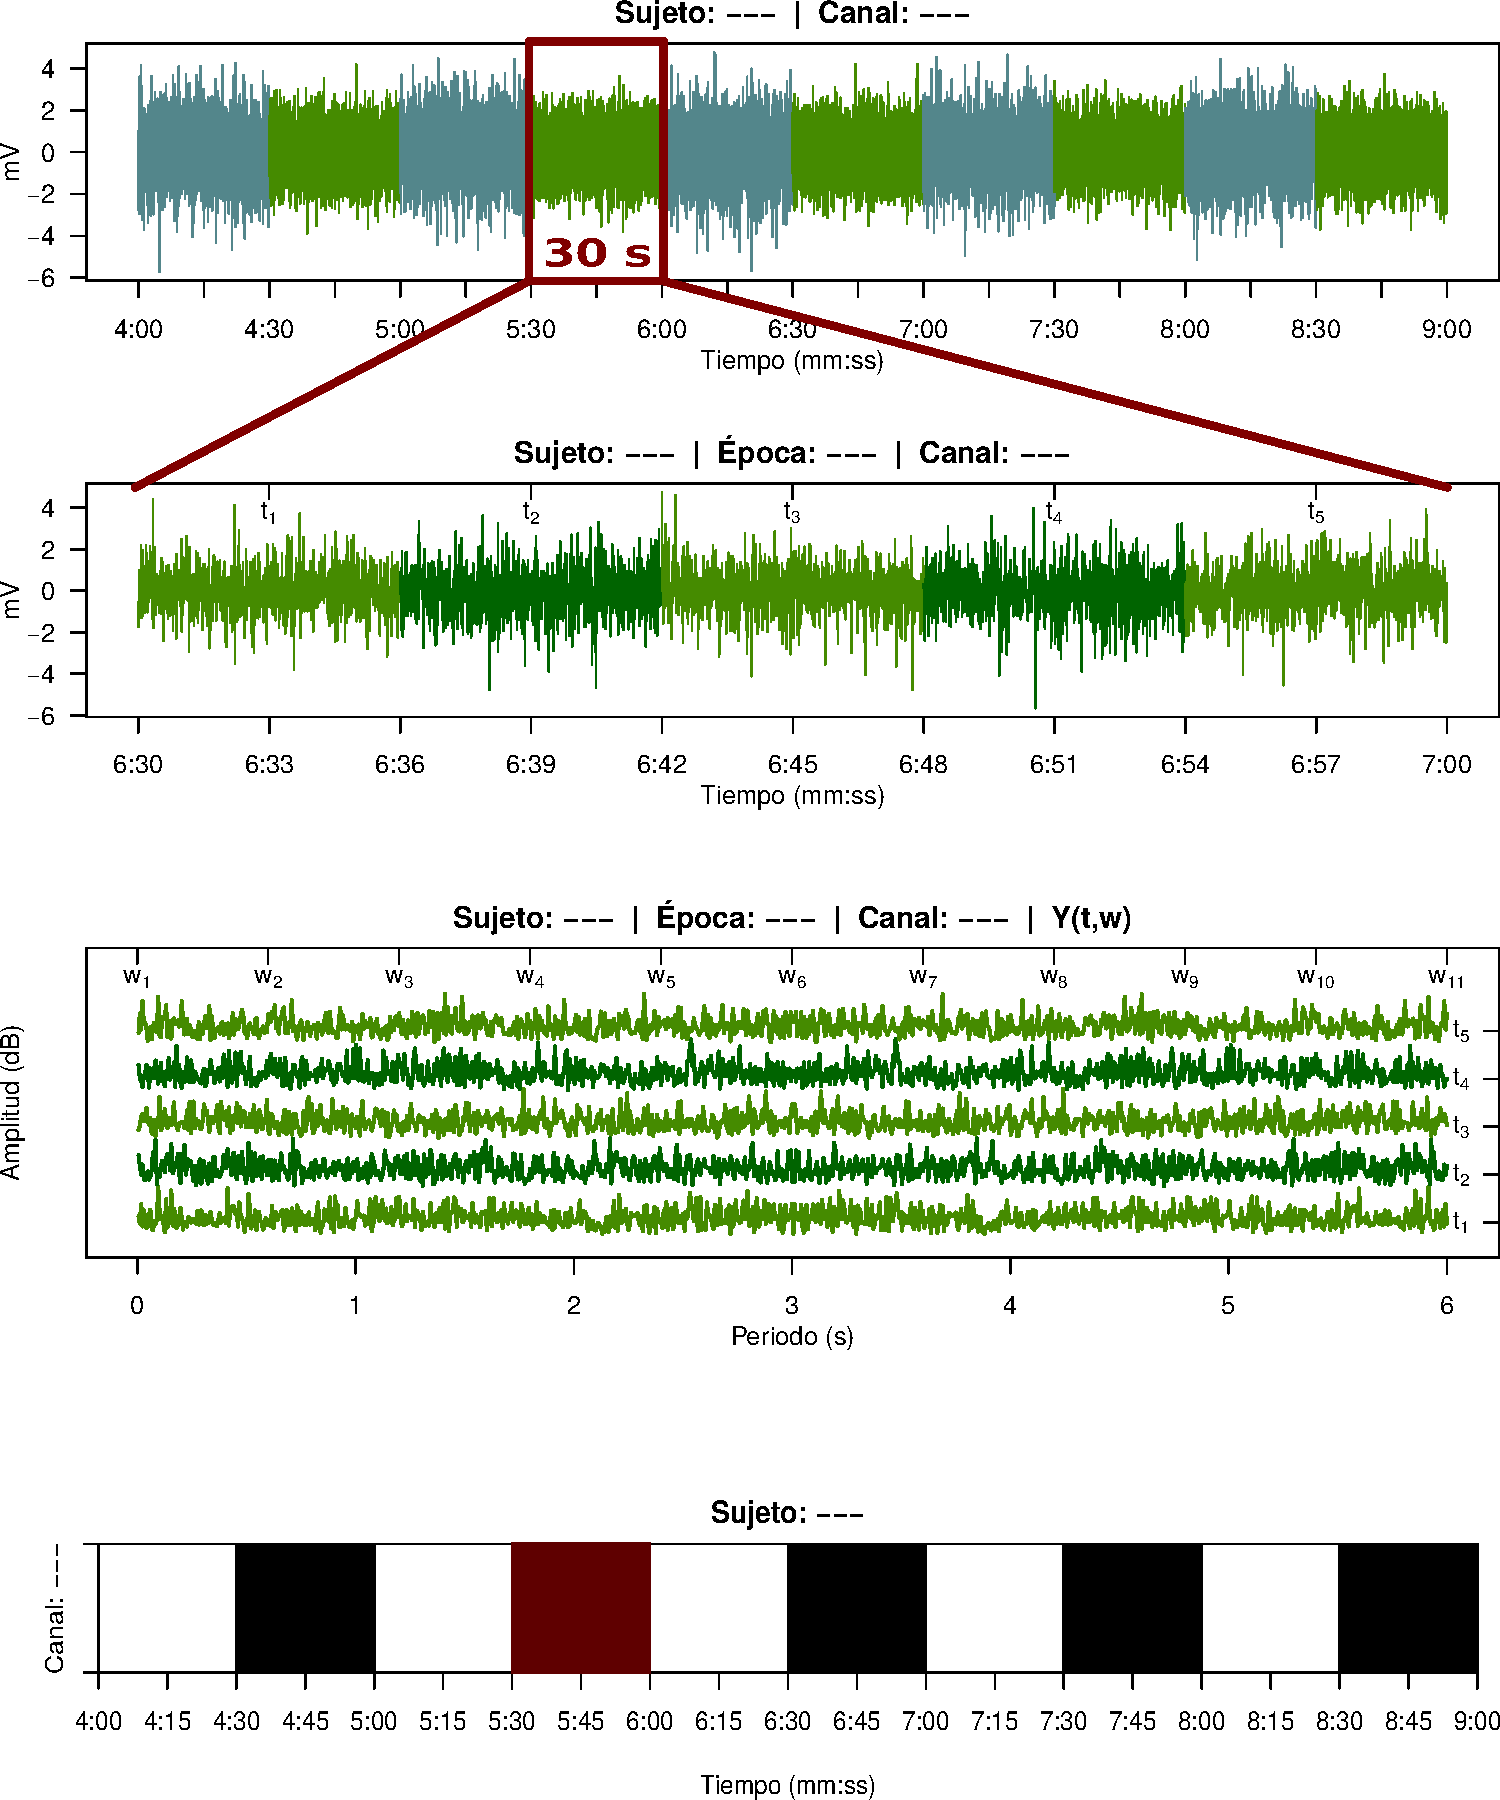
\includegraphics[width=0.7\linewidth]{./img_diagramas/psr_simple.pdf}
%\caption{Representación diagramática de la implementación en R de la prueba PSR. Se omite 
%filtrado previo mediante el algoritmo STL (ver texto).}
%\label{diagrama_psr}
%\end{figure}

Habiendo definido al estimador $Y$ según de esta forma en su versión discretizada (proceso resumido
en el gráfico \ref{diagrama_psr}), es posible definir criterios estadísticos para determinar la 
estacionariedad débil usando a $Y$. El primer caso es definir, como hipótesis nula, un modelo 
general
%
\begin{equation*}
H_0 : \hspace{1em} Y_{i,j} = \mu + \alpha_i + \beta_j + \gamma_{i,j} + \varepsilon_{i,j}
\end{equation*}
%
donde $\varepsilon$ son como se definieron anteriormente. Respecto a los otros parámetros, $\mu$ 
representa el promedio de $Y$ (así $\alpha$, $\beta$, $\gamma$ tienen media cero), $\alpha$ y 
$\beta$ son las \textit{variaciones} de $Y$ en el tiempo y las frecuencias, respectivamente, y 
$\gamma$ abarca las \textit{variaciones} no-lineales; $\gamma$ y $\varepsilon$ se diferencían en 
que por diseño se sabe que $\varepsilon_{i,j} \sim N(0,\sigma^{2})$, mientras que no se ha supuesto 
nada sobre $\gamma$.

Para determinar la estacionariedad se define, como hipótesis alterna, un modelo el $Y$ es 
efectivamente constante en el tiempo
%
\begin{equation*}
H_A : \hspace{1em} Y_{i,j} = \mu + \alpha_i + \varepsilon_{i,j}
\end{equation*}
%
posteriormente se prueba si se puede rechazar $H_0$ a favor de $H_A$; para ello se evalúan los 
estadísticos de el cuadro \ref{cantidades_psr} y se verifican las hipótesis 
$\nicefrac{S_{I+R}}{\sigma^{2}} = 0$ (para $\gamma=0$)  y $\nicefrac{S_T}{\sigma^{2}} = 0$ (para 
$\beta=0$).
Por cómo se construyeron, estos estadísticos tienen distribuciones $\chi^{2}$, con los grados de 
libertad indicados indicados en el cuadro.

\begin{table}
\centering
\bordes{1.1}
\begin{tabular}{llc}
\toprule
\multicolumn{2}{l}{{Estadístico}} & {Gr. de libertad} \\
\midrule
$S_T$ & $=J \sum_{i=1}^{I} \left( Y_{i,\bullet} - Y_{\bullet,\bullet} \right)^{2}$ 
& $I-1$ \\
$S_F$ & $= I \sum_{j=1}^{J} \left( Y_{\bullet,j} - Y_{\bullet,\bullet} \right)^{2}$ 
& $J-1$ \\
$S_{I+R}$ & $= \sum_{i=1}^{I} \sum_{j=1}^{J} 
\left( Y_{i,j} - Y_{i,\bullet} - Y_{\bullet,j} + Y_{\bullet,\bullet} \right)^{2}$ 
& $(I-1)(J-1)$ \\
%\midrule
\rowcolor{gris}
$S_{0}$ & $= \sum_{i=1}^{I} \sum_{j=1}^{J} 
\left( Y_{i,j} - Y_{\bullet,\bullet} \right)^{2}$ 
& $IJ -1$ \\
\midrulec
$Y_{i,\bullet}$ & $= \frac{1}{J} \sum_{j=1}^{J} Y_{i,j}$ & \\
$Y_{\bullet,j}$ & $= \frac{1}{I} \sum_{i=1}^{I} Y_{i,j}$ & \\
$Y_{\bullet,\bullet}$ & $= \frac{1}{I J} \sum_{i=1}^{I} \sum_{j=1}^{J} Y_{i,j}$ & \\
\bottomrule
\end{tabular}
\caption{Estadísticos involucrados en la prueba PSR}
\label{cantidades_psr}
\end{table}

Cabe mencionar que en la formulación original de la prueba de PSR se exploran algunas otros modelos 
que pueden ser verificadas usando el estimador $Y$ (cuadro \ref{modelos}); por ejemplo, los 
procesos \textbf{uniformemente modulados} (UM), que necesariamente pueden expresarse como 
$X(t) = S(t) X_0(t)$ donde $\{X_0(t)\}_{t\in T}$ un proceso débilmente estacionario, pueden 
modelarse usando $\gamma = 0$.

En esta caracterización, si se hace a $S$ constante ($\beta = 0$) es claro que los procesos UM 
contienen a los débilmente estacionarios; en cambio, si se hace a $f_0$ constante\footnote{Lo cual 
sólo es físicamente relevante si el proceso es a tiempo discreto} ($\alpha = 0$) entonces el 
proceso puede interpretarse como un PRB multiplicado en el tiempo por una función arbitraria.

\begin{table}
\centering
\begin{tabular}{lcc}
\toprule
{Modelo} & {Estacionario} & {UM} \\
\midrule
$H_0 : \hspace{.5em} Y_{i,j} = \mu + \alpha_i + \beta_j + \gamma_{i,j} + \varepsilon_{i,j}$
& \ding{55} & \ding{55} \\
$H_1 : \hspace{.5em} Y_{i,j} = \mu + \alpha_i + \beta_j + \varepsilon_{i,j}$ 
& \ding{55} & \ding{51} \\
$H_2 : \hspace{.5em} Y_{i,j} = \mu + \alpha_i + \varepsilon_{i,j}$ 
& \ding{51} & \ding{51} \\
$H_3 : \hspace{.5em} Y_{i,j} = \mu + \beta_j + \varepsilon_{i,j}$ 
& \ding{55} & \ding{51} \\
\bottomrule
\end{tabular}
\caption{Modelos que pueden ser contrastados usando la prueba PSR}
\label{modelos}
\end{table}

\subsubsection{Implementación}

Para poder usar efectivamente la prueba de PSR en el análisis de señales electrofisiológicas, ésta 
debe ser ejecutada por una computadora. 
Destaca que esta prueba ya se encuentra implementada para el software estadístico R \cite{R_citar}, 
dentro del paquete \texttt{fractal} \cite{R_fractal}; esta implementeación en particular será usada
en este trabajo, de modo que conviene estudiar su estructura.

%\begin{algorithm}
%  \caption{Prueba de Priestley-Subba Rao}
%  \label{influx}
%  \begin{algorithmic}[1]
%  \Require $p \in [0,1]$, $G$
%  \Ensure None \Comment{a test comment}
%  \For{$i = 0 \to 2^d-1$}\Comment{another test comment} 
%    \If{$n(\nu_i) = 0$}
%      \If{ $x < p$}  \Comment{$x$ is a normal distribution number in the range of $[0,1]$}
%      \State Occupy $v_i$ site with probablility $p$ 
%      \EndIf
%    \EndIf
%  \EndFor
%  \end{algorithmic}
%\end{algorithm}

\begin{algorithm}
%\SetAlgoLined
\DontPrintSemicolon
\KwData{$X = \left(x_1, x_2, \cdots, x_N \right)$}
\KwResult{p-valores para $S_{I+R} = 0$, $S_T = 0$, $S_F = 0$}
%initialization\;

%\For{$k = 1, \cdots$ \texttt{n.block}}{
$ X \leftarrow \left(x_1, x_2, \cdots, x_N \right)$\;
\For{$i = 1, \cdots$; $j=1, \cdots $}{
    $ U[i,j] \leftarrow \sum_{u = t-T}^{T} g(u) X[t-u] \exp\left(-\boldsymbol{i} \omega_j i\right)$ \;
}
\For{$i = 1, \cdots$; $j=1, \cdots $}{
    $ \widehat{f}[i,j] \leftarrow \sum_{u = t-T}^{T} w_\tau (u) \abso{U[i-u,j]}^{2}$ \;
}
$Y \leftarrow \log{\widehat{f}}$\;
\For{$i=1,\cdots, I$}{
    $Y_{i,\bullet} = \frac{1}{J} \sum_{j=1}^{J} Y_{i,j}$\;
}
\For{$j=1,\cdots, J$}{
    $Y_{\bullet,j} = \frac{1}{I} \sum_{i=1}^{I} Y_{i,j}$\;
}
$Y_{\bullet,\bullet} = \frac{1}{I J} \sum_{i=1}^{I} \sum_{j=1}^{J} Y_{i,j}$ \;

%}
%\displaystyle

\caption{Prueba de Priestley-Subba Rao}
%\label{stationarity}
\end{algorithm}


\begin{figure}
\centering
\begin{lstlisting}[caption={}]
Priestley-Subba Rao stationarity Test for datos
-----------------------------------------------
Samples used              : 3072 
Samples available         : 3069 
Sampling interval         : 1 
SDF estimator             : Multitaper 
  Number of (sine) tapers : 5 
  Centered                : TRUE 
  Recentered              : FALSE 
Number of blocks          : 11 
Block size                : 279 
Number of blocks          : 11 
p-value for T             : 0.4130131 
p-value for I+R           : 0.1787949 
p-value for T+I+R         : 0.1801353 
\end{lstlisting}
\caption{Resultado mostrado tras una ejecución de la función \texttt{stationarity}. 
%El parámetro \texttt{n.blocks} define la cantidad grupos disjuntos para los cuales se calculará 
%el estimador de la FDE.
%Cabe resaltar el antepenúltimo renglón (\texttt{p-value for T}), según el cual se puede
%aceptar o rechazar la hipótesis de estacionariedad débil. 
La FDE es referida como 'Spectral Density Function' (SDF).
}
\label{res_psr}
\end{figure}

%%%%%%%%%%%%%%%%%%%%%%%%%%%%%%%%%%%%%%%%%%%%%%%%%%%%%%%%%%%%%%%%%%%%%%%%%%%%%%%%%%%%%%%%%%%%%%%%%%%
%%%%%%%%%%%%%%%%%%%%%%%%%%%%%%%%%%%%%%%%%%%%%%%%%%%%%%%%%%%%%%%%%%%%%%%%%%%%%%%%%%%%%%%%%%%%%%%%%%%
%%%%%%%%%%%%%%%%%%%%%%%%%%%%%%%%%%%%%%%%%%%%%%%%%%%%%%%%%%%%%%%%%%%%%%%%%%%%%%%%%%%%%%%%%%%%%%%%%%%
%%%%%%%%%%%%%%%%%%%%%%%%%%%%%%%%%%%%%%%%%%%%%%%%%%%%%%%%%%%%%%%%%%%%%%%%%%%%%%%%%%%%%%%%%%%%%%%%%%%
